\documentclass[12pt, a4paper, titlepage]{article}
\usepackage[spanish]{babel}
\usepackage[utf8]{inputenc}
%%Imágenes
\usepackage{graphicx}
%%Colores de texto
\usepackage{xcolor}
\usepackage{colortbl}
%%Links
\usepackage[hidelinks]{hyperref}


\definecolor{guindapoli}{RGB}{102, 0, 51}
\definecolor{azulescom}{RGB}{0, 0, 102}
\definecolor{azulclaro}{RGB}{222, 232, 255}
\definecolor{azulfuerte}{RGB}{60, 150, 250}

\begin{document}
	
	%PORTADA
	\begin{titlepage}	
		
		\vspace*{-1.5in}
		
		\begin{figure}[htb]
			\begin{center}
				
\includegraphics[width=4cm]{./imagenes/logoipn.png}
			\end{center}
		\end{figure}
		
		\begin{center}
			
			\begin{LARGE}
				\textcolor{guindapoli}{INSTITUTO POLITÉCNICO NACIONAL}\\
			\end{LARGE}	
			
			\vspace*{0.2in}
			
			\begin{Large}
				\textcolor{azulescom}{ESCUELA SUPERIOR DE CÓMPUTO}\\
			\end{Large}		
			
			\vspace*{0.4in}
			
			\begin{large}
				Trabajo Terminal I.\\
			\end{large}
			
			\vspace*{0.2in}
			
			\begin{Large}
				\textbf{Autentificación Mediante Chaffing And Winnowing En El Protocolo HTTP}\\
			\end{Large}
			
			\vspace*{0.2in}
			
			\begin{large}
				2018-B003.\\
			\end{large}
			
			\vspace*{0.2in}
			
			\rule{80mm}{.1mm}\\
			\vspace*{0.1in}
			
			\begin{large}
				\begin{center}
					Integrantes:\\
					Carrillo Fernández Jerry\\
					Blancas Pérez Bryan Israel\\
					Morales González Diego Arturo\\
					Paredes Hernández Pedro Antonio\\
				\end{center}
			\end{large}
			
			\begin{large}
				Directores:\\
				Moreno Cervantes Axel Ernesto\\
				Díaz Santiago Sandra\\
			\end{large}
			
		\end{center}
	
	\end{titlepage}

	\begin{appendix}
		%%Índice
		\href{}{\renewcommand*\contentsname{{\textcolor{azulescom}{Índice.}}}}
		\tableofcontents
		\newpage
		%%índice de figuras
		\renewcommand*\listfigurename{{\textcolor{azulescom}{Índice de figuras.}}}
		\listoffigures
		\newpage
		%%Índice de tablas
		\newpage
		\renewcommand*\listtablename{{\textcolor{azulescom}{Índice de cuadros.}}}
		\listoftables
	\end{appendix}
	\newpage
	

	\section{\textcolor{azulescom}{Introducción.}}
		\subsection{Planteamiento del problema.}
			En la actualidad todos los usuarios de internet necesitan guardar contraseñas para sus distintas cuentas en las diferentes páginas web en las que ingresa ya que recordarlas es un problema que avanza constantemente. El uso de estas contraseñas son utilizadas principalmente en correos electrónicos y redes sociales por lo que el robo de las mismas puede poner en riesgo la seguridad del usuario, así como también, existe la tediosa tarea de ingresar usuario y contraseña en cada sesion. Las contraseñas son comúnmente utilizadas para el inicio de sesion y existen diferentes métodos de autentificación para dicho inicio como lo son biométricos. En nuestro proyecto nos enfocaremos más en el uso de text password en donde se autentificará el usuario por medio de una extensión de Google Chrome. Con ayuda de esta extensión resolveremos los problemas comentados anteriormente, dando así comodidad y seguridad al usuario que habilite la extensión.
		\newpage    
		\subsection{Justificación.}
			Los usuarios deben de guardar las contraseñas en medios fisicos o digitales y perderlos presenta un grave problema de seguridad. La gran mayoria de servicios web han implementado una solución la cual es recordar tu usuario y contraseña para que se pueda automaticamente acceder al servicio. Dicha solucion presenta cierta vulnerabilidad ya que los archivos donde se guarda la información se puede copiar y con ello replicarlo a otra computadora.
			En el cuadro No.1, se muestra una tabla donde se comparan los diferentes métodos de autentificación basándose en la simplicidad de su aplicación para el usuario (extraída del artículo Comparison of Authentication Methods on Web Resources). Donde: 1 – Bajo desempeño, 2 - Medio desempeño y 3 – Alto desempeño.
			
			\begin{table}[htb]
				\centering
				\resizebox{13cm}{!} {
					\begin{tabular}{l|l|l|l|l|l|l|l|}
						\cline{2-8}
						& Recordar & \begin{tabular}[c]{@{}l@{}}Otros\\ dispositivos\end{tabular} & Acciones & Facilidad & Tiempo & Errores & Recuperación \\ \hline
						\multicolumn{1}{|l|}{Contraseñas}                                                      & 1        & 3                                                            & 2        & 3         & 3      & 2       & 3            \\ \hline
						\multicolumn{1}{|l|}{Otros recursos}                                                   & 2        & 3                                                            & 3        & 3         & 3      & 3       & 2            \\ \hline
						\multicolumn{1}{|l|}{\begin{tabular}[c]{@{}l@{}}Contraseñas \\ gráficas\end{tabular}}  & 1        & 1                                                            & 2        & 3         & 3      & 2       & 3            \\ \hline
						\multicolumn{1}{|l|}{\begin{tabular}[c]{@{}l@{}}Contraseñas \\ dinamicas\end{tabular}} & 1        & 3                                                            & 2        & 2         & 3      & 2       & 2            \\ \hline
						\multicolumn{1}{|l|}{Tokens}                                                           & 3        & 1                                                            & 1        & 2         & 2      & 3       & 1            \\ \hline
						\multicolumn{1}{|l|}{Multivariación}                                                   & 1        & 1                                                            & 1        & 3         & 2      & 2       & 1            \\ \hline
						\multicolumn{1}{|l|}{Cryptografía}                                                     & 3        & 1                                                            & 1        & 1         & 1      & 2       & 1            \\ \hline
						\multicolumn{1}{|l|}{Biométricos}                                                      & 3        & 3                                                            & 2        & 3         & 2      & 2       & 1            \\ \hline
					\end{tabular}
				}
				\caption{Comparación de la aplicación en los distintos métodos de autentificación}
			\end{table}
			
			La tabla anterior concentra las siguientes caracteristicas:
			
			\begin{itemize}
				\item Recordar: Hace referencia a que tan complicado es que un usuario se acuerde de los datos necesarios para la autentificación. 
				\item Otros dispositivos: El usuario usa una entidad externa para facilitar su autentificación.
				\item Acciones: Hace referencia a que tantas acciones adicionales se deben de realizar para autentificarse.
				\item Facilidad: Simplicidad de tecnología.
				\item Tiempo: Cantidad de recursos temporales que consume el método de autentificación.
				\item Errores: Posibles errores durante la autentificación. 
				\item Recuperación: Denota la dificultad de recuperar la clave de acceso en caso de pérdida.
			\end{itemize}
				
			En el cuadro No.2 se muestra una tabla comparativa del nivel de seguridad en los distintos métodos de autentificación, donde 1 - baja seguridad, 2 – media seguridad y 3 – alta seguridad.
			
			\begin{table}[htb]
				\centering
				\resizebox{10cm}{!} {
					\begin{tabular}{l|l|l|l|l|}
						\cline{2-5}
						& \begin{tabular}[c]{@{}l@{}}Ataque por\\ fuerza bruta\end{tabular} & Observación & \begin{tabular}[c]{@{}l@{}}Hackeo\\ indirecto\end{tabular} & Phishing \\ \hline
						\multicolumn{1}{|l|}{Contraseñas}                                                      & 1                                                                 & 1           & 1                                                          & 1        \\ \hline
						\multicolumn{1}{|l|}{Otros recursos}                                                   & 2                                                                 & 2           & 3                                                          & 3        \\ \hline
						\multicolumn{1}{|l|}{\begin{tabular}[c]{@{}l@{}}Contraseñas \\ gráficas\end{tabular}}  & 1                                                                 & 1           & 2                                                          & 2        \\ \hline
						\multicolumn{1}{|l|}{\begin{tabular}[c]{@{}l@{}}Contraseñas \\ dinamicas\end{tabular}} & 2                                                                 & 3           & 2                                                          & 2        \\ \hline
						\multicolumn{1}{|l|}{Tokens}                                                           & 3                                                                 & 3           & 3                                                          & 3        \\ \hline
						\multicolumn{1}{|l|}{Multivariación}                                                   & 1                                                                 & 1           & 3                                                          & 3        \\ \hline
						\multicolumn{1}{|l|}{Cryptografía}                                                     & 3                                                                 & 3           & 3                                                          & 3        \\ \hline
						\multicolumn{1}{|l|}{Biométricos}                                                      & 3                                                                 & 3           & 1                                                          & 1        \\ \hline
					\end{tabular}
				}
			\caption{Comparación de la seguridad en los dstintos métodos de autentificación}
			\end{table}
		La tabla se enfoca principalmente en los siguientes problemas de seguridad: 
		
		\begin{itemize}
			\item Ataque por fuerza bruta: Se descifra el método de autentificación con una gran cantidad de intentos, usualmente generados por un programa.
			\item Observación: Cuando se intenta ver directamente los datos necesarios para la autentificación desde una distancia cercana hasta incluso usando binoculares, cámaras o algún otro dispositivo.
			\item Hackeo indirecto: El usuario confía sus datos del método de autentificación a terceros quienes pueden ser atacados. 
			\item Phishing: Hace referencia a programas que se hacen pasar por entidades confiables para interceptar los datos que desean.
		\end{itemize}
			
	\newpage
		\subsection{Objetivos.}
		\subsection{Metodología.}
		\subsection{Estado del Arte.}
	\newpage
	\section{\textcolor{azulescom}{Marco Teórico.}}
		\subsection{Formato a decidir.}
	\newpage
	\section{\textcolor{azulescom}{Análisis.}}
		\subsection{Prototipo I.}
			\subsubsection{Descripción.}
				En este prototipo se busca la creación de una extensión de Google Chrome, que sea capaz de interceptar una petición HTTP hecha por el navegador.
			\subsubsection{Herramientas a usar.}
				
				Para el desarrollo de software de este prototipo, ocuparemos las siguientes tecnologías debido a que nos facilitan el desarrollo y nos proporcionan lo necesario para lograr nuestro objetivo para este prototipo: 
				\paragraph {JavaScript. \\}
				JavaScript es considerado como el lenguaje de programación de HTML y de la web. Es un lenguaje de programación fácil de usar y muy versátil para el hámbito de la comunicación en redes.\cite{refJavaScript} 
				
				En el ambito del hardware utilizaremos los equipos de cómputo con los cuales contamos actualmente los integrantes, donde se especificaran a continuación: 
				
				\begin{table}[htb]
					\begin{tabular}{|p{3.5cm}||p{10cm}|}
						\rowcolor{guindapoli}
						\multicolumn{2}{|c|}{\textbf{\textcolor{white}{Equipo de hardware utilizado.}}}\\
						\hline
						\rowcolor{white}Nombre & Morales González Diego Arturo\\
						\hline
						\rowcolor{azulclaro}Marca & Asus\\
						\hline
						\rowcolor{white}Modelo & X550VC\\
						\hline
						\rowcolor{azulclaro}Procesador & Intel Core i5\\
						\hline
						\rowcolor{white}Tarjeta de video & NVidia GForce 720\\
						\hline
						\rowcolor{azulclaro}Memoria RAM & 12 GB\\
						\hline
						\rowcolor{white}Disco duro & 1TB\\
					\end{tabular}
				\end{table}
				
				\begin{table}[htb]
					\begin{tabular}{|p{3.5cm}||p{10cm}|}
						\rowcolor{guindapoli}
						\multicolumn{2}{|c|}{\textbf{\textcolor{white}{Equipo de hardware utilizado.}}}\\
						\hline
						\rowcolor{white}Nombre & Carrillo Fernández Gerardo\\
						\hline
						\rowcolor{azulclaro}Marca & HP\\
						\hline
						\rowcolor{white}Modelo & Pavilion g4\\
						\hline
						\rowcolor{azulclaro}Procesador & Intel Core i3\\
						\hline
						\rowcolor{white}Tarjeta de video & Intel Sandybridge Mobile\\
						\hline
						\rowcolor{azulclaro}Memoria RAM & 6 GB\\
						\hline
						\rowcolor{white}Disco duro & 500GB\\
					\end{tabular}
				\end{table}
				
				
			
			\subsubsection{Estudio de requerimientos.}
				
				\paragraph{Requerimientos Funcionales.\\ \\}
				
				{\setlength{\parindent}{12pt}
				\textbf{PI\_RF1. Interceptar petición HTTP.} La extensión deberá interceptar la petición HTTP del navegador, en cuanto el usuario realice alguna a través del navegador.\\

				\textbf{PI\_RF2. Deshabilitar extensión.} El usuario podrá deshabilitar la extensión, para que ésta no vigile su actividad en el navegador.\\
				
				\textbf{PI\_RF3. Habilitar extensión.} El usuario podrá habilitar la extensión, para que ésta vigile constantemente cuando éste realice una petición HTTP.
				}
				
				\paragraph{Requerimientos no Funcionales.\\ \\}
				{\setlength{\parindent}{12pt}
				
				\textbf{PI\_RNF1. Plataforma de implementación.} La extensión será implementada en el navegador Google Chrome.\\
				
				\textbf{PI\_RNF2. Versión del navegador} La extensión funcionará a partir de la versión 65.0.3325.181.\\
				
				\textbf{PI\_RNF3. Tecnologías para la interfaz de usuario} Para el sistema se hará uso de HTML, JavaScript, CSS, JSON.\\
				\footnote{Checar si es necesario especificar que debe estar habilitado JavaScript y si sería Funcional o No funcional}
				
				}
			
			\subsubsection{Reglas del negocio.}
				{\setlength{\parindent}{12pt}
					
				\label{PI_RN1}
				\textbf{PI\_RN1. Confidencialidad de la actividad web.} En cuando el cliente lo indique por medio de la IU, la extensión deberá dejar de vigilar la actividad que el usuario realice en el navegador. De igual forma, si el usuario indicara dejar de vigilar la actividad web, la extensión así lo hará.\\
					
				}\newpage
	\newpage
	\section{\textcolor{azulescom}{Desarrollo.}}
		\subsection{Prototipo I.}
			\subsubsection{Diagrama de casos de uso.}

				Diagrama de casos de uso general para el prototipo I.
				\begin{figure}[htb]
					\begin{center}
						\label{fig1} 
						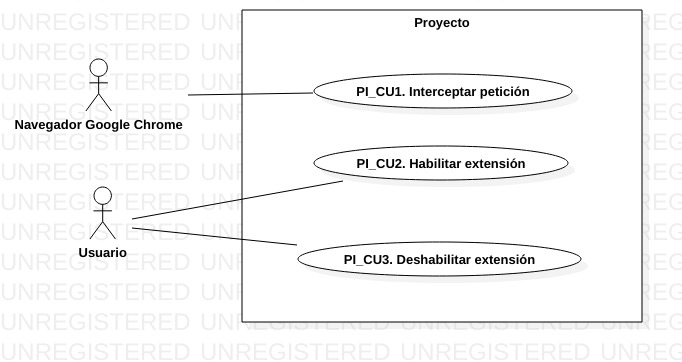
\includegraphics[width=17cm]{./imagenes/UCD_1.jpg}
						\caption{Diagrama de casos de uso.}
					\end{center}
				\end{figure}\newpage	
					
			\subsubsection{Descripción de casos de uso.}
				\footnote{EL actor es el navegador?}
			
				%%DESCRIPCIÓN PI_CU1
				\begin{table}[htb]
				\begin{tabular}{ |p{3.5cm}||p{9.5cm}|}
					\hline
					\rowcolor{guindapoli}
					\multicolumn{2}{|c|}{\textbf{\textcolor{white}{Caso de uso: PI\_CU1. Interceptar petición.}}}\\
					\hline
					\rowcolor{azulfuerte}Concepto & Descripción\\
					\hline
					\cellcolor{azulclaro}Actor & 
					Navegador de Google Chrome.\\ 
					\hline
					\cellcolor{azulclaro}Propósito &
					Este caso de uso permite a la extensión interceptar una petición HTTP, realizada por el navegador Google Chrome por medio de algún agente (sistema o usuario) externo a éste.\\
					\hline
					\cellcolor{azulclaro}Entradas &
					Petición HTTP realizada por el navegador.\\
					\hline
					\cellcolor{azulclaro}Salidas &
					Petición HTTP cachada.\\
					\hline
					\cellcolor{azulclaro}Pre-condiciones&
					Algún agente externo (Sistema o usuario) ha ordenado al navegador mandar una petición HTTP.\\
					\hline
					\cellcolor{azulclaro}Post-condiciones&
					La extensión, deberá de interceptar la petición para poder modificarla.\\
					\hline
					\cellcolor{azulclaro}Reglas del negocio&
					-\\
					\hline
					\cellcolor{azulclaro}Errores &
					La petición no se pudo interceptar. \newline La petición no es tipo HTTP.\\					
					\hline
				\end{tabular}
				\caption[DCU: PI\_CU1]{Descripción CU: PI\_CU1}
				\end{table}
				
				\paragraph{... Trayectoria Principal ...}
				\begin{enumerate}
					\item \textbf{\textit{El Usuario}} o \textbf{\textit{El Sistema Externo}} realiza una petición HTTP en el navegador Google Chrome.\\
					\item \textbf{\textit{La Extensión}} intercepta la petición antes de que salga a red.\\
					\item \textbf{\textit{La Extensión}} puede modificar el contenido de la petición. \\
					\item \textbf{\textit{La Extensión}} deja salir a red la petición.
				\end{enumerate}
				\paragraph{... Fin de la Trayectoria Principal ...}
				
				\paragraph{... Trayectoria Alternativa 1 ...}
				\begin{enumerate}
					\item \textbf{\textit{El Usuario}} o \textbf{\textit{El Sistema Externo}} no realiza una petición HTTP en el navegador Google Chrome.\\
					\item \textbf{\textit{La Extensión}} ignora la petición.					
				\end{enumerate}
				\paragraph{... Fin de la Trayectoria Alternativa 1 ...}
				
				\paragraph{... Trayectoria Alternativa 2 ...}
				\begin{enumerate}
					\item \textbf{\textit{El Usuario}} o \textbf{\textit{El Sistema Externo}} realiza una petición HTTP en el navegador Google Chrome.\\
					\item \textbf{\textit{La Extensión}} no puede interceptar la petición antes de que salga a red.\\
					\item \textbf{\textit{La Extensión}} notifica que hubo un error al intentar interceptar la petición. 
				\end{enumerate}
				\paragraph{... Fin de la Trayectoria Alternativa 2 ...}
				
				\newpage
				%%DESCRIPCIÓN PI_CU2
				\begin{table}[htb]
				\begin{center}
				\begin{tabular}{ |p{3.5cm}||p{9.5cm}|}
					\hline
					\rowcolor{guindapoli}
					\multicolumn{2}{|c|}{\textbf{\textcolor{white}{Caso de uso: PI\_CU2. Habilitar extensión.}}}\\
					\hline
					\rowcolor{azulfuerte}Concepto & Descripción\\
					\hline
					\cellcolor{azulclaro}Actor & 
					Usuario.\\ 
					\hline
					\cellcolor{azulclaro}Propósito &
					Este caso de uso, permite al usuario habilitar a la extensión, para que ésta sea capaz de ver todas las peticiones que realiza el navegador.\\
					\hline
					\cellcolor{azulclaro}Entradas &
					Indicación de habilitar extensión, mediante interfaz de usuario.\footnote{Si sería esta la entrada?}\\
					\hline
					\cellcolor{azulclaro}Salidas &
					Ninguna.\\
					\hline
					\cellcolor{azulclaro}Pre-condiciones&
					El usuario debe de haber instalado la extensión en Google Chrome y haber permitido su ejecución.\\
					\hline
					\cellcolor{azulclaro}Post-condiciones&
					La extensión verá todas las peticiones que realice el navegador.\\
					\hline
					\cellcolor{azulclaro}Reglas del negocio&
					\hyperref[PI_RN1]{PI\_RN1.}\\
					\hline
					\cellcolor{azulclaro}Errores &
					No se puede iniciar la vigilancia de la extensión.\\
					
					\hline
				\end{tabular}
				\caption[DCU: PI\_CU2]{Descripción CU: PI\_CU2}
				\end{center}
				\end{table}
				
				\paragraph{... Trayectoria Principal ...}
				\begin{enumerate}
					\item \textbf{\textit{El usuario}} da click en el ícono de la extensión \textbf{insert icon}.
					\item \textbf{\textit{El usuario}} da click en el botón \textbf{insert button} "Habilitar extensión".
					\item \textbf{\textit{La extensión}} empieza a vigilar las peticiones que se realicen a través del navegador.
				\end{enumerate}
				\paragraph{... Fin de la Trayectoria Principal ...}
				
				\paragraph{... Trayectoria Alternativa 1 ...}
				\begin{enumerate}
					\item \textbf{\textit{El usuario}} da click en el ícono de la extensión \textbf{insert icon}.
					\item \textbf{\textit{El usuario}} da click en el botón \textbf{insert button} "Deshabilitar extensión".
					\item \textbf{\textit{La extensión}} muestra mensaje de error "La extensión ya está deshabilitada".
				\end{enumerate}
				\paragraph{... Fin de la Trayectoria Alternativa 1 ...}
				
				\paragraph{... Trayectoria Alternativa 2 ...}
				\begin{enumerate}
					\item \textbf{\textit{El usuario}} no encuentra el ícono de la extensión \textbf{insert icon}.
				\end{enumerate}
				\paragraph{... Fin de la Trayectoria Alternativa 2 ...}
				
				\newpage
				
				\newpage
				%%DESCRIPCIÓN PI_CU3
				\begin{table}[htb]
				\begin{center}
				\begin{tabular}{ |p{3.5cm}||p{9.5cm}|}
					\hline
					\rowcolor{guindapoli}
					\multicolumn{2}{|c|}{\textbf{\textcolor{white}{Caso de uso: PI\_CU3. Deshabilitar extensión.}}}\\
					\hline
					\rowcolor{azulfuerte}Concepto & Descripción\\
					\hline
					\cellcolor{azulclaro}Actor & 
					Usuario.\\ 
					\hline
					\cellcolor{azulclaro}Propósito &
					Este caso de uso, permite al usuario deshabilitar a la extensión, para que ésta ignore todas las peticiones que se realicen por medio del navegador.\\
					\hline
					\cellcolor{azulclaro}Entradas &
					Indicación de deshabilitar extensión, mediante interfaz de usuario.\footnote{Si sería esta la entrada}\\
					\hline
					\cellcolor{azulclaro}Salidas &
					Ninguna.\\
					\hline
					\cellcolor{azulclaro}Pre-condiciones&
					El usuario debe de haber instalado la extensión en Google Chrome y haber permitido su ejecución.\\
					\hline
					\cellcolor{azulclaro}Post-condiciones&
					La extensión dejará de ver todas las peticiones que realice el navegador.\\
					\hline
					\cellcolor{azulclaro}Reglas del negocio&
					\hyperref[PI_RN1]{PI\_RN1.}\\
					\hline
					\cellcolor{azulclaro}Errores &
					No se puede detener la vigilancia de la aplicación.\\
					\hline
				\end{tabular}
				\caption[DCU: PI\_CU3]{Descripción CU: PI\_CU3}
				\end{center}
				\end{table}
			
				\paragraph{... Trayectoria Principal ...}
				\begin{enumerate}
					\item \textbf{\textit{El usuario}} da click en el ícono de la extensión \textbf{insert icon}.
					\item \textbf{\textit{El usuario}} da click en el botón \textbf{insert button} "Deshabilitar extensión".
					\item \textbf{\textit{La extensión}} deja de vigilar las peticiones que se realicen a través del navegador.
				\end{enumerate}
				\paragraph{... Fin de la Trayectoria Principal ...}
				
				\paragraph{... Trayectoria Alternativa 1 ...}
				\begin{enumerate}
					\item \textbf{\textit{El usuario}} da click en el ícono de la extensión \textbf{insert icon}.
					\item \textbf{\textit{El usuario}} da click en el botón \textbf{insert button} "Habilitar extensión".
					\item \textbf{\textit{La extensión}} muestra mensaje de error "La extensión ya está habilitada".
				\end{enumerate}
				\paragraph{... Fin de la Trayectoria Alternativa 1 ...}
				
				\paragraph{... Trayectoria Alternativa 2 ...}
				\begin{enumerate}
					\item \textbf{\textit{El usuario}} no encuentra el ícono de la extensión \textbf{insert icon}.
				\end{enumerate}
				\paragraph{... Fin de la Trayectoria Alternativa 2 ...}
			
				\newpage
				%FIN DE LA DESCRIPCIÓN DE CASOS DE USO
				
			\subsubsection{Diagrama de flujo.}
			\subsubsection{Flujo de datos.}
			\subsubsection{Diagrama de clases.}
			\subsubsection{Diagrama de secuencia.}
			\subsubsection{Interfaz de usuario.}
			\subsubsection{Requisitos de diseño.}
	%Para agregar una cita en el documento se usa \cite{refKey}, por automático los ordena conforme se van agregando
	\begin{thebibliography}{20}
		\bibitem{refJavaScript} https://javascript.info/intro \\
		
	\end{thebibliography}		
\end{document}

